\section{The Control Panel web application}
In the modular architecture of IPOL all the modules are able to work standalone since they are servers implementing Stateless webservices. However, a coordinated view from both the functional and administrative point of view is needed.

The Control Panel web application offers a unified interface to configure and administrate the platform. For example, the Editors can remove unused experiments for the archive or add new images to a demo.

At the present moment, the control panel provides a navigation menu option for each module , 
so you can interact with each modile using the webservices they provide.

The Integrated view of the whole sistem is not ready , but it will be built uppon the pieces that manage each module. This 

\subsection{Status navigation menu option}
The user will be able to monitor if the modules are running and in what machine they are runing.This will be done using the ping or stats ws provided by the different modules.
It's also possible to add tests experiments to the testing demo.
All modules should run under proxy module.

\subsection{Archive navigation menu option}
The Archive module is responsible for storing the experiments made bay users. When a user select a file of his own instead of using ono of the files proposed by the demo, This file is uploaded and used to run the demo bt Demo module, then teh result of this execution is sent to Archive module to be stored. Some demos have 40000 experiments.

The user will be presented with a list of demos that have experiments in the archive module, the user will be able to delete these demos from the archive, with all their related info.

When the user selects a demo, he will be presented with a list of all the experiments of the demo (we\'ll use pagin), and each experiment will display its information, files included. A user can delete experiments and files. If a file is deleted, all demos that use this file will also be deleted.


\subsection{Blobs navigation menu option}
The Blobs module is responsible for storing the images used as default images for runing the demos.
The user will be presented with a list of demos that have blobs in the blob module,
He will be able to remove, add, edit and delete blobs from a demo.
Not ready yet. Partially implemented.

\subsection{Demoinfo navigation menu option}
Allows you to manage the demoinfo module.


\subsection{Demo Dispatcher navigation menu option}
Not ready yet.

\subsection{Demo Runner navigation menu option}
Not ready yet.

\subsection{Proxy navigation menu option}
The ointegration between proxy and demoinfo is done, but this section remains beacuse it would be interesting to be able to get some stats from the proxy module and present them to the user of the control panel, perhaps not to the editors, but to the admin.
If this funcionality is not requiered, this menu entry should be deleted.
Not ready yet.

\subsection{user manual navigation menu option}
A user manual for the editors that will use the control panel, could be as simple as a pdf link or a help page.
Not ready yet.

\subsection{Demos navigation menu option}
The Demo execution system consists od a Demo Dispatcher module, a Demo Runner module and a DemoInfo module.
Integrated view of the previous sections whith the demo system.
Not ready yet.

% The Control Panel Module 
\subsection{Tecnical information}
In this section we'll discuss the project's structure and how to deploy it in diferent enviroments
This module is implemented using Django framework so we'll explain some basic information about how to configure a django web app.
The use or virtualenv is recomended.

\subsection{Project structure}
This is the Django project structure.
One project ipolwebapp with one app named controlpanel.


\begin{figure}[!ht]
\centering
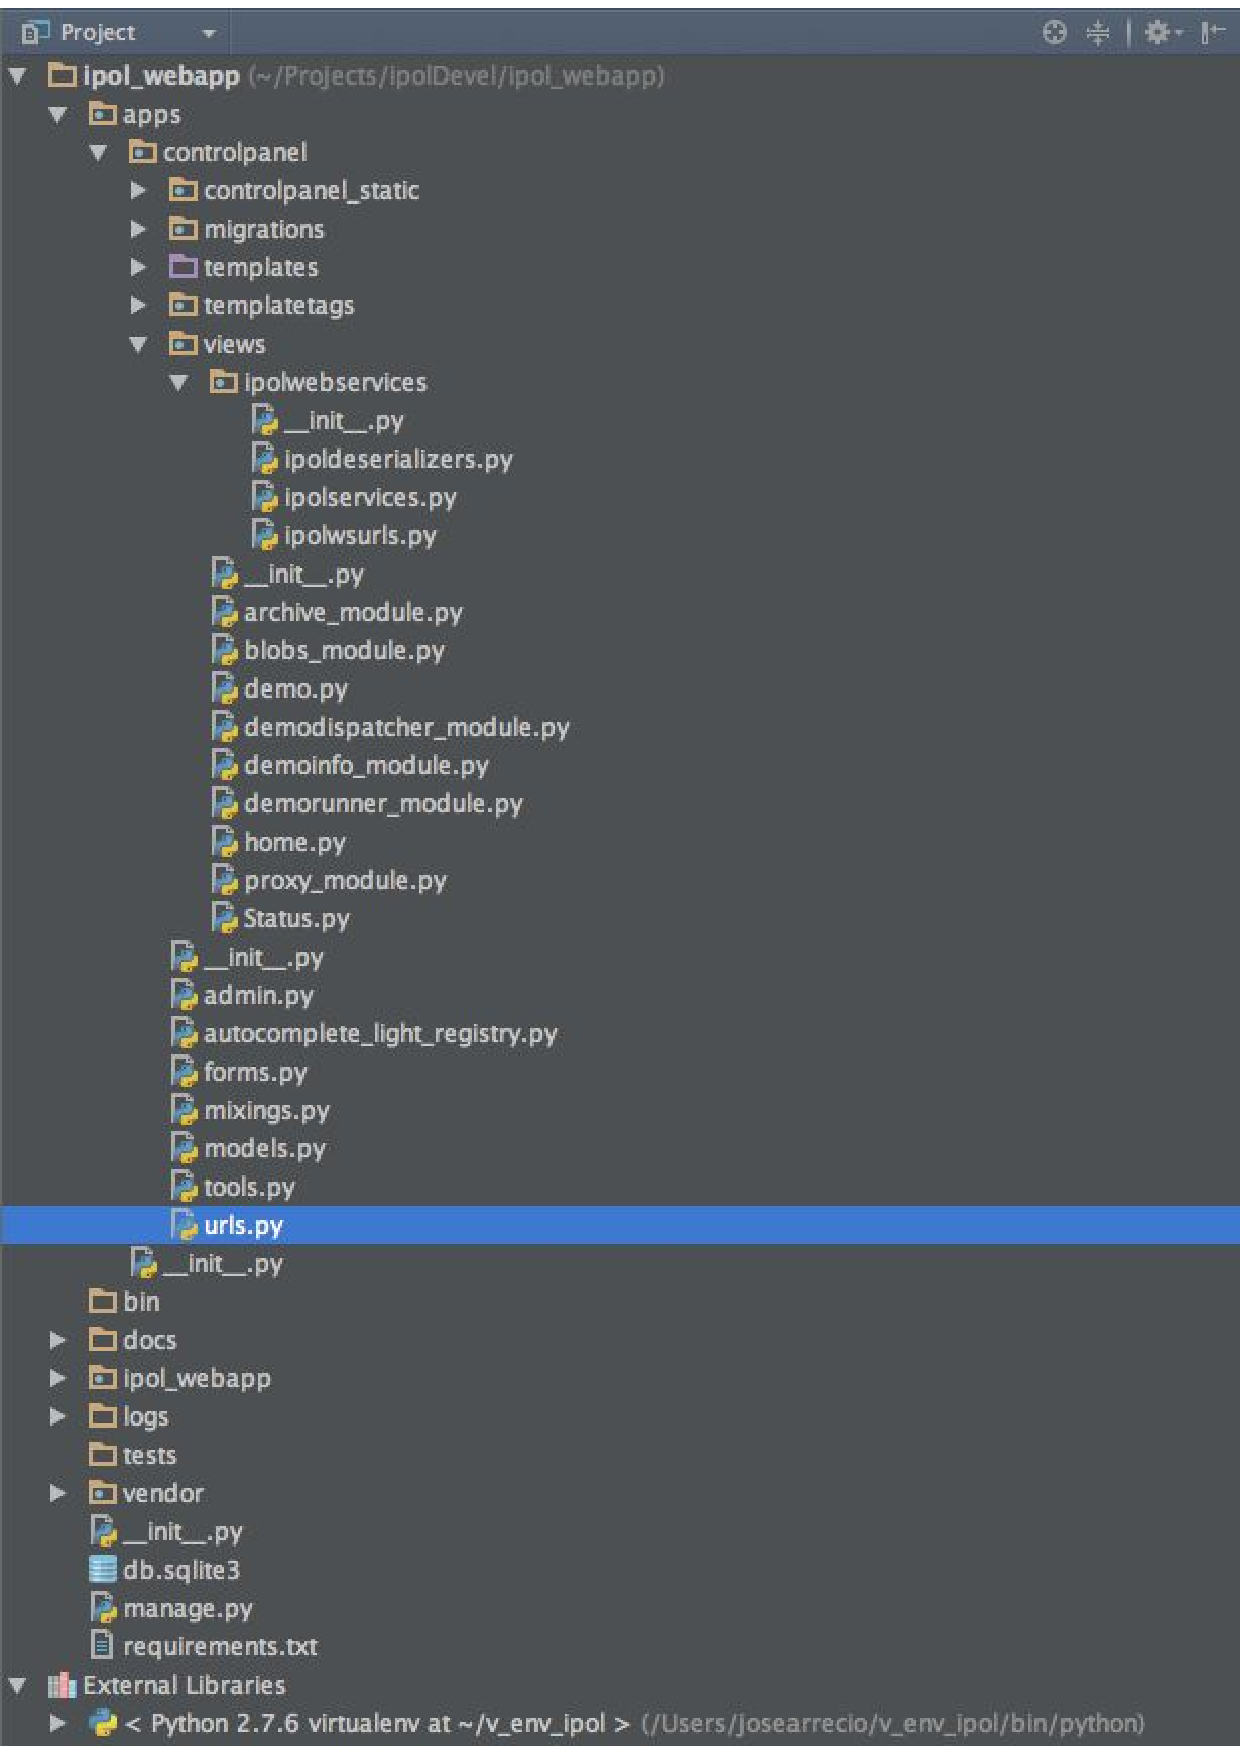
\includegraphics[width=0.5\columnwidth]{control_panel/images/ipol_webapp_project.pdf}
\caption{Project Structure (Pycharm IDE tool, wich I recommend). } 
\label{fi:project_structure}
\end{figure}
Describe folders.

\begin{itemize}
\item  apps
This folder is where you the apps you create for the ipol\_webapp project should go.There is only one app at this time, controlpanel.
\item  apps\/controlpanel
Is the folder of the controlpanel app, it contaisn folder and some import files , like models.py that contains the controlpanel app model, beacuse controlpanel only uses the services provided by the modules, it does not have a model, its does not store any data from the modules in its DB (it does stores user prfiles information so you can login and more stuff so the app can work )
\item  apps\/controlpanel\/controlpanel\_static
Staic files go in this folder, js, css etc.
\item  apps\/controlpanel\/templates
Templates for each module, each module has a folder.
\item  apps\/controlpanel\/views
Here you have the business logic code. you will find a .py file for each module
\item  apps\/controlpanel\/views\/ipolwebservices
Here you have code that allows controlpanel to access the diferent webservices, 
ipolwsurls.py contains the name of the services that controlpanel will need
ipolservices.py contains functions that make the call using the service names provided by ipolwsurls.py to the proper module.
ipoldeserializers.py provides code to deserialize the json returned by the ws and conver it to python objects. This is donde for complex objects like lists. They are reused in many places. 
\item  bin
Empty at the present moment, contains deployment scripts
\item  docs
Howto docs
\item  ipol\_webapp
The project folder, contains the main configuration files.
\item  tests
Empty at the present moment,Unit tests shoul go here.
\item  vendor
External apps that require adaptation to project. (you cant just install them with pip and use.)
The only app that has been adapted is allauth. Its installed with pip like the rest, but in vendors I provide adaptos and templates so I can customize allauth.
\end{itemize}

Describe important/configuration files

\begin{itemize}
\item  ipol\_webapp\/settings.py
This is the main configuration file, it contains the list of apps installed (INSTALLED\_APPS), the configuration of django and all the apps included in the project (if they need any configuration), the configuration of i18n translations, the logers, the static and media folders,the templates, the databases, the middleware, the cache (memcache is configured but not used) and at the begining of the file there's a first section that looks for the name of the machine the app is running on, and depending on the hostname it loads settings for the local environment or the development environment.

If you want to run this app locally, you must add the hostname of your machine to the local\_machines list, 
to run on a dev machine,add the hostname of your machine to dev\_machines.

Local and development machines can runn wih debug = True and no cache, and they can use the runserver provided by django

For a production enviroment, you must add the hostname of your machine to the production\_machines list,  DEBUG must be false, the use of memcache is recommended, and you must serve staicfiles properly. A proper server must be provided (apache naginx gunicorn...etc there are many recepies for a django deployment), YOU MUST NEVER USE RUNSERVER for production.
 

\item  ipol\_webapp\/urls.py
It contais a list of url patterns, 
A simple example:
\begin{lstlisting}[language=Python,firstnumber=1]
url(r'^status/', StatusView.as_view(), name="ipol.cp.status")
\end{lstlisting}
When http://hostname/status/ is entered in the webbrowser, Django will look in url.py for a match, an then the code in StatusView will run and prepare the data that will be shown in the template defined in the StatusView Class.
ipol.cp.status is the name I use to generate this url in my code or templates. this way you can avoid using hardcoded urls.

\item  ipol\_webapp\/wsgi.py
Automaticly generated by django when project was created.

\item  ipol\_webapp\/apps\/controlpanel\/urls.py
Controlpanel urls.

\item  db.sqlite3
The database.

\item  requirements.txt
The Requirements file, it contains the pip packages the project needs to satify dependencies. And commented you'll find tips telling you how to install them. 
\begin{lstlisting}[language=Python,firstnumber=1]
pip install -r "requirements.txt"
\end{lstlisting}

\item  tests
Unit tests, not implemented yet.

\item  vendor
Customized django apps, only allauth (for user login ) at the present moment. Theres adaptes and templates to get the allauth app inegrated in the ipol\_webapp project.

\end{itemize}


\subsubsection{Apps}
This section describes the external apps ipolwebapp uses and why it needs them. I wil not discuss the django.contrib apps, only external aps

\begin{itemize}

\item  autocomplete\_light
\url{https://django-autocomplete-light.readthedocs.org/en/master/}
This package allows you to enable autocompletes quickly and properly in a django project.

\item  rest\_framework
\url{http://www.django-rest-framework.org/}
Django REST framework is a powerful and flexible toolkit for building Web APIs. It is used in this project in ipolserializers.py and only to serialize / deserialize data.

\item  allauth
\url{https://github.com/pennersr/django-allauth}
Integrated set of Django applications addressing authentication, registration, account management as well as 3rd party (social) account authentication.

\item  crispy\_forms
\url{https://github.com/maraujop/django-crispy-forms}
django-crispy-forms provides you with a 
\begin{lstlisting}[language=Python,firstnumber=1]
|crispy 
\end{lstlisting}
 filter and 
\begin{lstlisting}[language=Python,firstnumber=1]
 
\end{lstlisting}
tag that will let you control the rendering behavior of your Django forms in a very elegant and DRY way. Have full control without writing custom form templates. All this without breaking the standard way of doing things in Django, so it plays nice with any other form application.

\end{itemize}


\subsubsection{Model}
The model of ipolwebapp's controlpanel app.
There is none, no data is stored by controlpanel app.
Note that the other apps in the project do have a model (for example, allauth need to store users etc so you can login).


\subsubsection{Learning Django}
Django is a high-level Python Web framework that encourages rapid development and clean, pragmatic design. Built by experienced developers, it takes care of much of the hassle of Web development, so you can focus on writing your app without needing to reinvent the wheel. It’s free and open source.

Django usefull information:

Django project - \url{https://www.djangoproject.com/}

Class based views in django - \url{http://ccbv.co.uk/}

\subsection{Deployment}
For testing you can run it using runserver as described in ipol\_Webapps docs folder
But for a production enviroment you should not use runserver. Apache or nginx as a reverse proxy and gunicorn is recomended.

This is how a deploymant is made

\begin{itemize}
\item  ssh to server 
\item  load virtualviroment (if using virtualenv)
\begin{lstlisting}[language=Python,firstnumber=1]
(ipol_virtual_env)user@prodmachine:/Users/myuser$
cd /Users/myuser/myvenvs/ipol_virtual_env
source bin/activate
(ipol_virtual_env)user@prodmachine:/Users/myuser/myvenvs/ipol_virtual_env$
cd /var/www/Ipol_webap
(ipol_virtual_env)user@prodmachine:/var/www/Ipol_webap$ 
python manage.py 
\end{lstlisting}
\item  get code from git
\item  migrations
This is to aply changes in the model or installed app's models, so changes are aplied to the database without having to delete and recreate the database.
\begin{lstlisting}[language=Python,firstnumber=1]
python manage.py migrate  --list
python manage.py migrate
\end{lstlisting}
\item  Start/ restart aplication server
\item  Start/ restart static files aplication server (if any)

\end{itemize}



\subsubsection{Test Enviroment}
For the test enviroment you can use the testing server that comes with django.

\begin{lstlisting}[language=Python,firstnumber=1]
 (ipol_virtual_env)user@devmachine:/var/www/Ipol_webap$ 
 python manage.py migrate  --list
 
 (ipol_virtual_env)user@devmachine:/var/www/Ipol_webap$ 
 python manage.py collectstatic
 
 (ipol_virtual_env)user@devmachine:/var/www/Ipol_webap$ 
 nohup python manage.py runserver 0.0.0.0:8000 &./dev/null &
\end{lstlisting}


\subsubsection{Production Enviroment}
The production eviroment requires a secure deployment, yo cannot user runserver. An example could be apache as reverse proxy and for serving static content and gunicorn as application server. Nginx is also a popular application server used for Django apps.


Django deployment tutorial:

\url{http://pyvideo.org/video/236/pycon-2010--django-deployment-workshop}


Django-Nginx-Gunicorn setup:

Nginx - \url{http://nginx.org/en/docs/}
Gunicorn - \url{http://docs.gunicorn.org/en/latest/deploy.html}


Django-Nginx setup:

Django-Nginx - \url{http://uwsgi-docs.readthedocs.org/en/latest/tutorials/Django_and_nginx.html}


Django-Apache setup:

Apache2 - \url{https://httpd.apache.org/}
Apache mod\_wsgi - \url{http://thecodeship.com/deployment/deploy-django-apache-virtualenv-and-mod_wsgi/}



\subsubsection{Manage static content in Production Enviroment }
Here describe how to setup static content with apache or nginx. find tutorials

Django project:

\url{http://blog.yourlabs.org/post/30382323418/surviving-djangocontribstaticfiles-or-how-to}

To collect static files run from the project folder:

\begin{lstlisting}[language=Python,firstnumber=1]
 (ipol_virtual_env)user@prodmachine:/var/www/Ipol_webap$ 
 python manage.py collectstatic
\end{lstlisting}


\subsubsection{Contol Panel modification example}

In this section I will show you how to add a new page to the controlpanel app, 
It will be a simple hello world page, but I will try to explain in detail all the process.
You fill find many Django tutorials, but this example is based in the actuall code you may need to maintain.

This Hello World page will display a "hello world" message on the screen, but it will also present the navbar, so the user can navigate in the controlpanel app. 
It will also need a helloworld entry in the navbar so the user can navigate to this newly created page. The django app will have to be able to recognize that the user requested the hello world page, execute the business code and present the result in a template so he user can see the hellow world page.
We will also want the user to be loged in the app to be able to view this page.
 
The first step would be create an entry in the urls.py file of the controlpanel app.
There you will add something like:

\begin{lstlisting}[language=Python,firstnumber=1]
url(r'^hello_world/', HelloWorldView.as_view(),
 name="ipol.cp.helloworld"),
\end{lstlisting}

The first part is the regex that django will try to match with the url the user accesed on the webbrowser, if the user is asking for hello\_world/ , then it will run the code stored in HelloWorldView class (we have to create and import this class for the url to worl. )
I would recomend to go to the views/ folder and create a file helloworl.py and in there:

\begin{lstlisting}[language=Python,firstnumber=1]
class HelloWorldView(NavbarReusableMixinMF,TemplateView):
	pass
\end{lstlisting}

Well discuss this class further on, right now we are only creating the class so we can import it in urls.py.

The url name , ipol.cp.helloworld must be unique and we'll use this to generate the url to our helloworld page in the templetes, this way we avoid things like: 

\begin{lstlisting}[language=Python,firstnumber=1]
<a href="hello_world/">
\end{lstlisting}

Instead we will use the django url resolvers, using the url template tag :

\begin{lstlisting}[language=Python,firstnumber=1]
<a href="">
\end{lstlisting}

To add this link to the navbar, you have to know the structure of the templates, they all extend a base template, 

\begin{lstlisting}[language=html,firstnumber=1]

\end{lstlisting}

and this base.html includes a footer.html

\begin{lstlisting}[language=html,firstnumber=1]
        <!-- footer Section -->
        
\end{lstlisting}

In this footer.html file you will find the navbar, there you will need to add a menu item for your new helloworld page.

\begin{lstlisting}[language=html,firstnumber=1]
{#   helloworld   #}
<li class="nav-item 
	 
		active 
	">
	<a href="">
		
	</a>
</li>
\end{lstlisting}

Let me point out a few things about django templates adn the footer.html file, 

\begin{itemize}
\item  request.session.menu == 'menu-helloworld' is to check if a sesion variable named menu
is equal to  'menu-helloworld', this way we mark this navbar menu option as active.
The value of the menu session variable is set in the HelloWorldView view.

\item  the trans tag is for translations, the i18n setup is not complete for this app, but in case you need translations you can add django-rosetta and configure it.
Anyway it's a good practice to use these tags, so when you add translations your html is ready.

\item  the url tag with the url name ipol.cp.helloworld generates the link to our hello world page.

\end{itemize}

Now we need to have a look at the HelloWorldView(NavbarReusableMixinMF,TemplateView) Class,
The first thing to notice is that it inherits from NavbarReusableMixinMF and TemplateView.
This means our class will have the functions of those classes it inherits from.

\begin{itemize}
\item  NavbarReusableMixinMF is defined in controlpanel/mixings.py, this class has a function allauth\_guests that returns the variable ALLAUTH\_GESTS defined in settings.py , this is to know if the app allows allauth user logings or not.
\item  TemplateView is a django generic view, this web \url{http://ccbv.co.uk/} is a good reference. templateView expects a template.
\end{itemize}

Django generic view are good because they let you reuse code (DRY) and 
remove a lot of boilerplate code.
\url{https://docs.djangoproject.com/es/1.9/topics/class-based-views/intro/}

so now we can complete the HelloWorldView Class

\begin{lstlisting}[language=Python,firstnumber=1]
class HelloWorldView(NavbarReusableMixinMF,TemplateView):
	template_name = "hw/hello_world.html"

	@method_decorator(login_required)
	def dispatch(self, *args, **kwargs):
		self.request.session['menu'] = 'menu-helloworld'
		return super(HelloWorldView, self).dispatch(*args, **kwargs)


	def get_context_data(self, **kwargs):
		#get context
		context = super(HelloWorldView, self).get_context_data(**kwargs)
		#send context vars for template
		context['hw_message'] = "My Hello World Message!!!"
		return context
		
	def my_get_hw_message(self, **kwargs):
		return "My Hello World Message!!!"
		
\end{lstlisting}

Let me point out a few things:

\begin{itemize}
\item  template\_name needs a html templete, we will need to create "hw/hello\_world.html"
\item  dispatch is decoreted with @method\_decorator(login\_required), 
this ensures we are loged in.

\item  get\_context\_data is a method inherited from TemplateView, and we can override it to add context variables that we will be able to access in the template (hello\_world.html)

\item  my\_get\_hw\_message is a function that retuns a string, this is also accessible from hello\_world.html, so for this case is a better solution than overriding get\_context\_data.
But sometimes you cannot encapsulete functionallity in such an easy way, that is why just passing variable to the template using get\_context\_data is easier.

\end{itemize}


Having completed the url, and te view, the only thing that remains is the template.
we can create hello\_world.html in the folder .../controlpanel/templates/hw/hello\_world.html

\begin{lstlisting}[language=html,firstnumber=1]





    Hello World







<h1>Ipol Webap Helo World</h1>

  <p>Ipol Webap , for the integration / management of 
  the modules demo, archive. blobs ...</p>
  <p>display context variable that contains 
  my hw message: {{ hw_message }}</p>
  <p>display my hw message using my 
  my_get_hw_message function : {{ view.my_get_hw_message }}</p>






		
\end{lstlisting}

\begin{itemize}
\item  load loads tags we need, staticfiles is for accessing staic content and i18n is for the translation tags
\item  we display the message using the context data and the my\_get\_hw\_message function of the HelloWorldView view.

\end{itemize}



